
%%%%%%%%%%%%%%%%%%%%%%% file typeinst.tex %%%%%%%%%%%%%%%%%%%%%%%%%
%
% This is the LaTeX source for the instructions to authors using
% the LaTeX document class 'llncs.cls' for contributions to
% the Lecture Notes in Computer Sciences series.
% http://www.springer.com/lncs       Springer Heidelberg 2006/05/04
%
% It may be used as a template for your own input - copy it
% to a new file with a new name and use it as the basis
% for your article.
%
% NB: the document class 'llncs' has its own and detailed documentation, see
% ftp://ftp.springer.de/data/pubftp/pub/tex/latex/llncs/latex2e/llncsdoc.pdf
%
%%%%%%%%%%%%%%%%%%%%%%%%%%%%%%%%%%%%%%%%%%%%%%%%%%%%%%%%%%%%%%%%%%%


\documentclass[runningheads,a4paper]{llncs}

\usepackage{amssymb}
\setcounter{tocdepth}{3}
\usepackage{graphicx}

\usepackage[portuguese]{babel}
\usepackage[utf8]{inputenc}

\usepackage{url}
\urldef{\mailsa}\path|{alfred.hofmann, ursula.barth, ingrid.haas, frank.holzwarth,|
\urldef{\mailsb}\path|anna.kramer, leonie.kunz, christine.reiss, nicole.sator,|
\urldef{\mailsc}\path|erika.siebert-cole, peter.strasser, lncs}@springer.com|    
\newcommand{\keywords}[1]{\par\addvspace\baselineskip
\noindent\keywordname\enspace\ignorespaces#1}

\begin{document}

\mainmatter  % start of an individual contribution

% first the title is needed
\title{Desenho e implementação de um jogo distribuído na Internet}

% a short form should be given in case it is too long for the running head
\titlerunning{Desenho e implementação de um jogo distribuído na Internet}

% the name(s) of the author(s) follow(s) next
%
% NB: Chinese authors should write their first names(s) in front of
% their surnames. This ensures that the names appear correctly in
% the running heads and the author index.
%
\author{Oliveira Rui, Araujo Paulo, Costa Orlando}
%
\authorrunning{liveira Rui, Araujo Paulo, Costa Orlando}
% (feature abused for this document to repeat the title also on left hand pages)

% the affiliations are given next; don't give your e-mail address
% unless you accept that it will be published
\institute{Universidade do Minho, Gualtar, Portugal\\
\url{http://www.uminho.pt}}

%
% NB: a more complex sample for affiliations and the mapping to the
% corresponding authors can be found in the file "llncs.dem"
% (search for the string "\mainmatter" where a contribution starts).
% "llncs.dem" accompanies the document class "llncs.cls".
%

\toctitle{Lecture Notes in Computer Science}
\tocauthor{Authors' Instructions}
\maketitle


\begin{abstract}
The abstract should summarize the contents of the paper and should
contain at least 70 and at most 150 words. It should be written using the
\emph{abstract} environment.
\keywords{We would like to encourage you to list your keywords within
the abstract section}
\end{abstract}


\section{Introdução}

\section{Diferenças da especificação}

O protocolo implementado segue o proposto no enunciado com duas diferenças.
Na lista de argumentos de uma PDU tinha o tamanho do parâmetro. Estava previsto que este tamanho apenas tivesse 1 bytes, mas isto não era suficiente por exemplo no caso do bloco de musica. Portanto modificou-se para 2 bytes.
Adicionou-se também um tipo de PDU de controlo para os servidores fecharem os sockets em segurança. 

\section{Implementação}

\subsection{Protocolo}


\begin{figure}
\centering
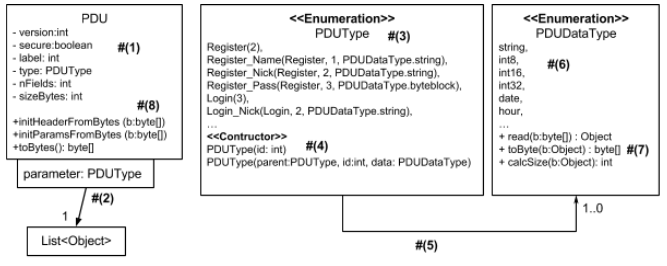
\includegraphics[height=6.2cm]{UDP.png}
\caption{Diagrama UMP da interpretação de PDU}
\label{fig:diagram-pdu}
\end{figure}

Para a abstração dos Bits, foi criada a classe PDU, que é capaz de criar as PDU’s e depois transformas em Bytes e também inicializar-se através de array de Bytes.
Internamente existem os parâmetros do cabeçalho da PDU [\#(1)] (versão, segurança, label, tipo da PDU, número de campos e tamanho tamanho total dos campos em Bytes), toda esta informação pode ser consultada com os seus respetivos métodos.
Para guardar os campos da PDU, utiliza-se um Map [\#(2)] onde a chave é o tipo do campo e o valor é uma lista de valores. Uma lista porque a mesma PDU pode ter varias campos com o mesmo tipo como é o exemplo de uma questão que têm varias respostas.

A Enumeração PDUType [\#(3)] é uma enumeração hierárquica, isto é: existem os valores de origem que representam o tipo da PDU como por exemplo: Register, Login, Replay. Depois existem os valores que representam os campos, como por exemplo: Register\_Name ou Register\_Nick.
A Diferença entre estes dois está no construtor utilizada [\#(4)]. No caso do construtor de um campo podemos reparar que recebe um tipo de dados (PDUDataType).

A enumeração PDUDataType [\#(6)] tem todos os tipos de dados que o PDU suposta, e aqui ficam implementadas as funções de leitura e conversão para arrays de bytes.
Desta forma é fácil a adição de novos tipos de dados.

O diagrama \ref{fig:diagram-pdu} UML explica o funcionamento da interpretação do campos do PDU (função initParamsFromBytes).

\begin{figure}
\centering
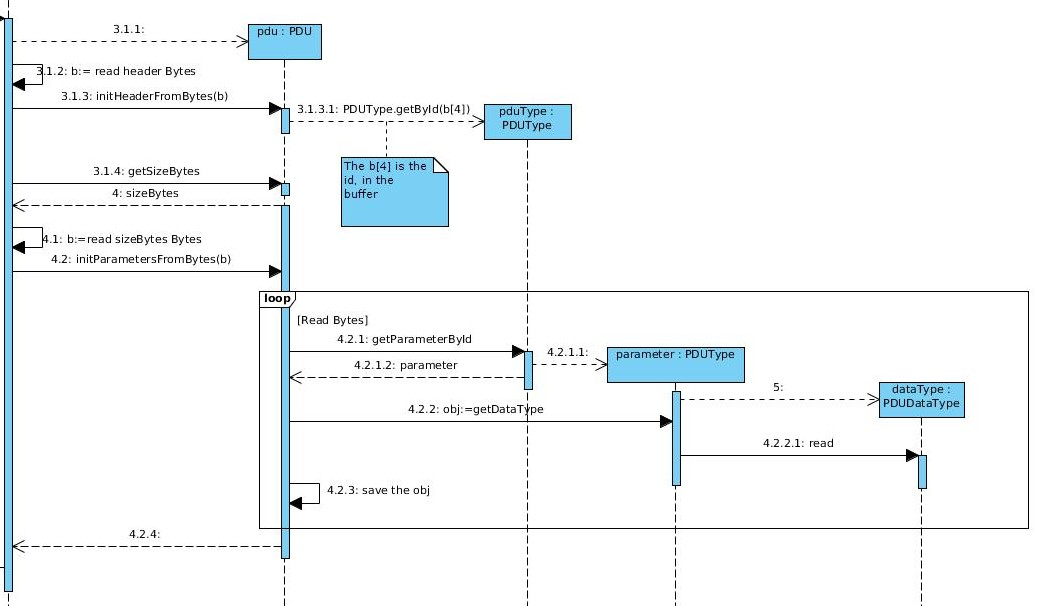
\includegraphics[height=6.2cm]{PDU_interpretation.jpg}
\caption{Diagrama UMP da interpretação de PDU}
\label{fig:diagram-pdu}
\end{figure}

\subsection{Cliente}

\subsection{Servidor}

O Servidor é responsável guardar a informação sobre do sistema tais como os desafios e utilizadores existentes. Por outro lado o servidor também é responsável por partilhar o seu conhecimento com os outros servidores.
No arranque o servidor cria 2 threads, um deles para atender clientes, e outro para atender outros  servidores 

A arquitetura geral de um servidor posso ser vista no diagrama \ref{fig:diagram-arq-geral}.

\begin{figure}
\centering
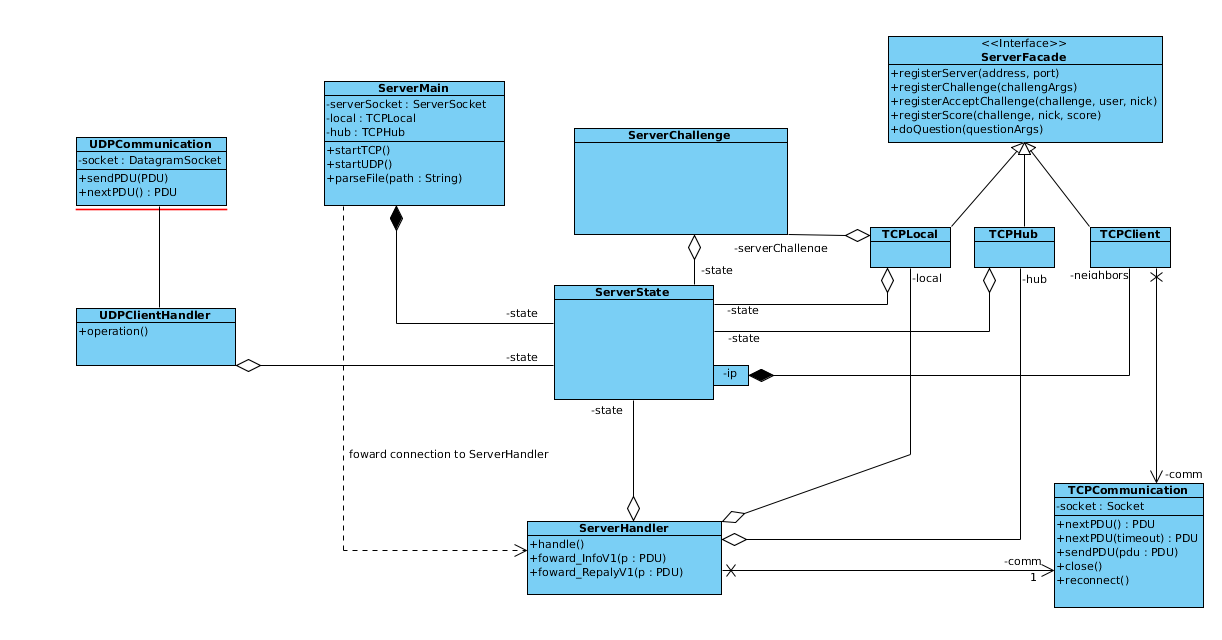
\includegraphics[height=6.2cm]{arq-geral.png}
\caption{Diagrama UML da arquitetura do servidor}
\label{fig:diagram-arq-geral}
\end{figure}


\subsubsection{Dados Guardados}

Toda a informação relativa ao actual estado de um servidor são guardos na classe ServerState:
\begin{itemize}
  \item Utilizadores identificados por o seu nick
  \item Sessões, guardam os utilizadores identificados por o seu ip actual
  \item Utilizadores globais, para guarda o ranking global do sistema.
  \item Desafios identificados por o seu nome
  \item Questões para criar novos desafios, identificados por o seu ip
  \item Servidores vizinhos poder comunicar.
\end{itemize}

No caso dos desafios cada desafio tem: o ranking atual dos utilizadores inscritos nesse desafio, os utilizadores e servidores subscritos e as questões selecionadas.

\subsubsection{Atender Clientes}

Um pedido vindo de um cliente é reencaminhado para a class UDPClientHandler, aqui mediante o tipo de desafio, é realizada as regras de negocio correspondente e enviada uma resposta para o cliente.

Existem alguns pedidos do cliente que podem gerar que o servidor que esteja a antender tenha que informar os restantes servidores como por exemplo: makeChallenge, que inicia um desafio e irá ser explicado de seguida. 
Iniciar desafio

Quando um makeChallenge e gerado, o sistema cria uma nova thread que terá um temporalizador para correr às horas pretendidas. Quando esta thread inicia o seu processo confirma que existem pessoas suficientes no desafio, caso não existam cancela o desafio. Caso esteja tudo bem continua e envia a primeira pergunta.

As perguntas ao longo do desafio são enviadas para todos os clientes subscritos e para todos os servidores subscritos, depois cada um destes servidores reencainhará para os clientes finais.

\subsubsection{Atender Servidores}

O processo de atender servidores é semelhante ao de atender clientes.  Os pedidos são interpretados na class ServerHandler, esta class mediante os parametros existentes irá executar a logica de negocio necessária.
O negocio está implementado em 3 classes distintas: TCPLocal, TCPHub e TCPClient. Cada uma destas implementam a interface ServerToServerFacade que especifica todos os métodos existentes no negocio da aplicação (diagrama \ref{fig:diagram-facades}).

Cada uma das implementações implementa o negocio de forma diferente:
\begin{itemize}
\item TCPLocal aplica as regras de negocio na propria maquina.
\item TCPClient envia um pedido a um servidor para aplicar aquele método.
\item TCPHub aplica as regras de negocio a todos os servidores chamando o TCPClient de cada servidor.
\end{itemize}

O socket que permite a comunicação entre servidores é terminado com um timeout parameterizavel.

\begin{figure}
\centering
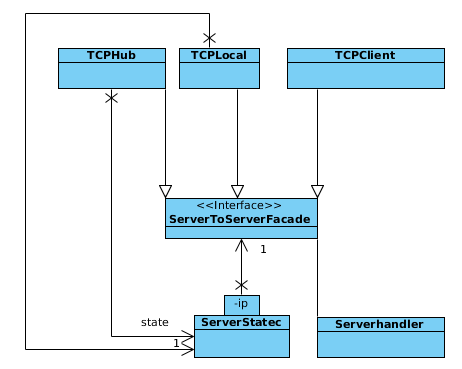
\includegraphics[height=6.2cm]{facades.png}
\caption{Diagrama UML da arquitetura do servidor}
\label{fig:diagram-facades}
\end{figure}


\subsubsection{Informar Servidores Vizinhos}

Para comunicar com outros servidores utiliza-se ou TCPHub ou TCPClient mediante as necessidades.
O TCPClient que irá fazer é abrir um socket se necessário, e enviar uma PDU do tipo INFO com a informação pretendida.

\section{Testes Realizados}

De forma a validar o trabalho realizado, foram efetuados alguns testes. Os testes foram realizados com a utilização de um router, sendo que foi necessária a sua configuração de modo a que, a partir do MAC Address dos pc’s conectados, fossem atribuídos IP’s escolhidos por nós. Através da criação de várias instâncias de clientes e servidores nos computadores conectados, é possível criar uma simulação de um ambiente de comunicação real no qual existem servidores dedicados que recebem os pedidos de ligação dos respetivos clientes.

\subsection{Registo de um Utilizador}

\begin{itemsize}

\item IP Servidor: 127.0.0.2
\item IP Cliente: 127.0.0.75

\end{itemsize}

Cliente > REGISTER joao rodrigues 123

I'm[/127.0.0.75] sending to [/127.0.0.2] PDU: PDU,parameters:{REGISTER_PASS=[[B@1d56ce6a], REGISTER_NAME=[joao], REGISTER_NICK=[rodrigues]}

I'm[/127.0.0.2] sending to [/127.0.0.75] PDU: PDU,parameters:{REPLY_OK=[0]}

Servidor > OK

\subsection{Participação em Desafio}

\begin{itemsize}

\item IP Servidor: 127.0.0.1
\item IP Cliente1: 127.0.0.66
\item IP Cliente2: 127.0.0.69

\end{itemsize}

Cliente1 > MAKE_CHALLENGE Circo 2015-05-02 15:00

I'm[/127.0.0.66] sending to [/127.0.0.1] PDU: PDU,parameters:{MAKE_CHALLENGE_CHALLENGE=[Circo], MAKE_CHALLENGE_HOUR=[15:00], MAKE_CHALLENGE_DATE=[2015-05-02]}

I'm[/127.0.0.1] sending to [/127.0.0.66] PDU: PDU,parameters:{REPLY_CHALLE=[Circo], REPLY_DATE=[2015-05-02], REPLY_HOUR=[15:00]}

Servidor >  Desafio: Circo Data: 2015-05-02 Hora: 15:00

Cliente2 > ACCEPT_CHALLENGE Circo

I'm[/127.0.0.69] sending to [/127.0.0.1] PDU: PDU,parameters:{ACCEPT_CHALLENGE_CHALLENGE=[Circo]}

I'm[/127.0.0.1] sending to [/127.0.0.69] PDU: PDU,parameters:{REPLY_OK=[0]}

Servidor > OK


\end{document}
